\selectlanguage{italian}

La fisica delle particelle studia i costituenti fondamentali della materia e le interazioni fra loro. La materia è costituita da particelle e campi, i quali sono associati alle interazioni e causano le forze attraverso le quali interagiscono le particelle: le interazioni sono mediate da particolari particelle, dette \textit{bosoni di gauge}. Le particelle fondamentali, come i quarks e l'elettrone, possono essere considerati puntiformi ($ \lesssim 10^{-16}\,\text{cm} $, mentre un nuclide $ \sim 10^{-13}\,\text{cm} $).

\paragraph{Particelle}

Solo quattro particelle sono stabili, di cui sono due sono fondamentali: il protone, il neutrone, l'elettrone ed il neutrino. Le altre particelle decadono rapidamente verso le particelle stabili, ed infatti sono tendenzialmente più massive di quest'ultime. A causa dell'instabilità, queste particelle non si trovano in natura, ma possono essere prodotte sperimentalmente usando fasci di particelle incidenti con sufficiente energia (superiore alla rest energy delle particelle da produrre).\\
Attualmente, le particelle fondamentali più massive scoperte sono il bosone $ W $ ($ 80.4\gev/c^2 $), il bosone $ Z $ ($ 91.2\gev/c^2 $), il bosone di Higgs ($ 125\gev/c^2 $) ed il quark top ($ 173\gev/c^2 $). Ciascuna di queste particelle è circa un centinaio di volte più pesante del protone; per produrle sono necessarie altissime energie, mentre per studiarle è necessario sondare distanze piccolissime: dal principio di Heisenberg, se $ \Delta x \ll 1\fm $, allora $ \Delta p \gg 200\mev/c $.

\paragraph{Interazioni}

Tutte le interazioni tra particelle sono dovute allo scambio di particelle mediatrici. Ad oggi si conoscono solo quattro interazioni fondamentali: quella gravitazionale, quella debole, quella elettromagnetica e quella forte. Si pensa, però, che nelle prime frazioni di secondo dell'universo queste fossero unificate (almeno quelle forte, debole ed elettromagnetica): si parla di \textit{Grand Unification Theory} (GUT), secondo la quale, col trascorrere del tempo ed il diminuire della temperatura dell'universo, le interazioni si siano gradualmente separate, fino ad avere quelle che osserviamo oggi. Le predizioni della GUT, però, rimangono tuttora inosservate sperimentalmente: le principali sono il decadimento del protone su scale lunghissime, l'esistenza di monopoli magnetici e l'esistenza di dipoli elettrici fondamentali, ovvero particelle che, sebbene puntiformi, presentano un'asimmetria di carica.

\paragraph{Modello Standard}

All'inizio del Novecento si avevano evidenze sperimentali soltanto dell'elettrone, del fotone e dei nuclei atomici, ma nel giro di un secolo si è arrivati a sviluppare un modello che spiegasse la formazione di tutte le particelle della materia a partire da quelle fondamentali: il \textit{Modello Standard} (Fig. \ref{standard-model}). Questo è appunto un modello, e non una teoria: mentre la seconda dà spiegazioni esatte dei dati sperimentali e ne predice di nuovi, un modello è soltanto un'approssimazione desunta dagli esperimenti, dunque deve essere integrato man mano che questi procedono, e non ha potere predittivo. Il Modello Standard è uno dei modelli più solidi mai sviluppati e ad oggi non è stato ancora messo in crisi, sebbene non spieghi varie cose: ad esempio, la massa dei neutrini e la divisione dei fermioni in generazioni.

\begin{figure}
	\centering
	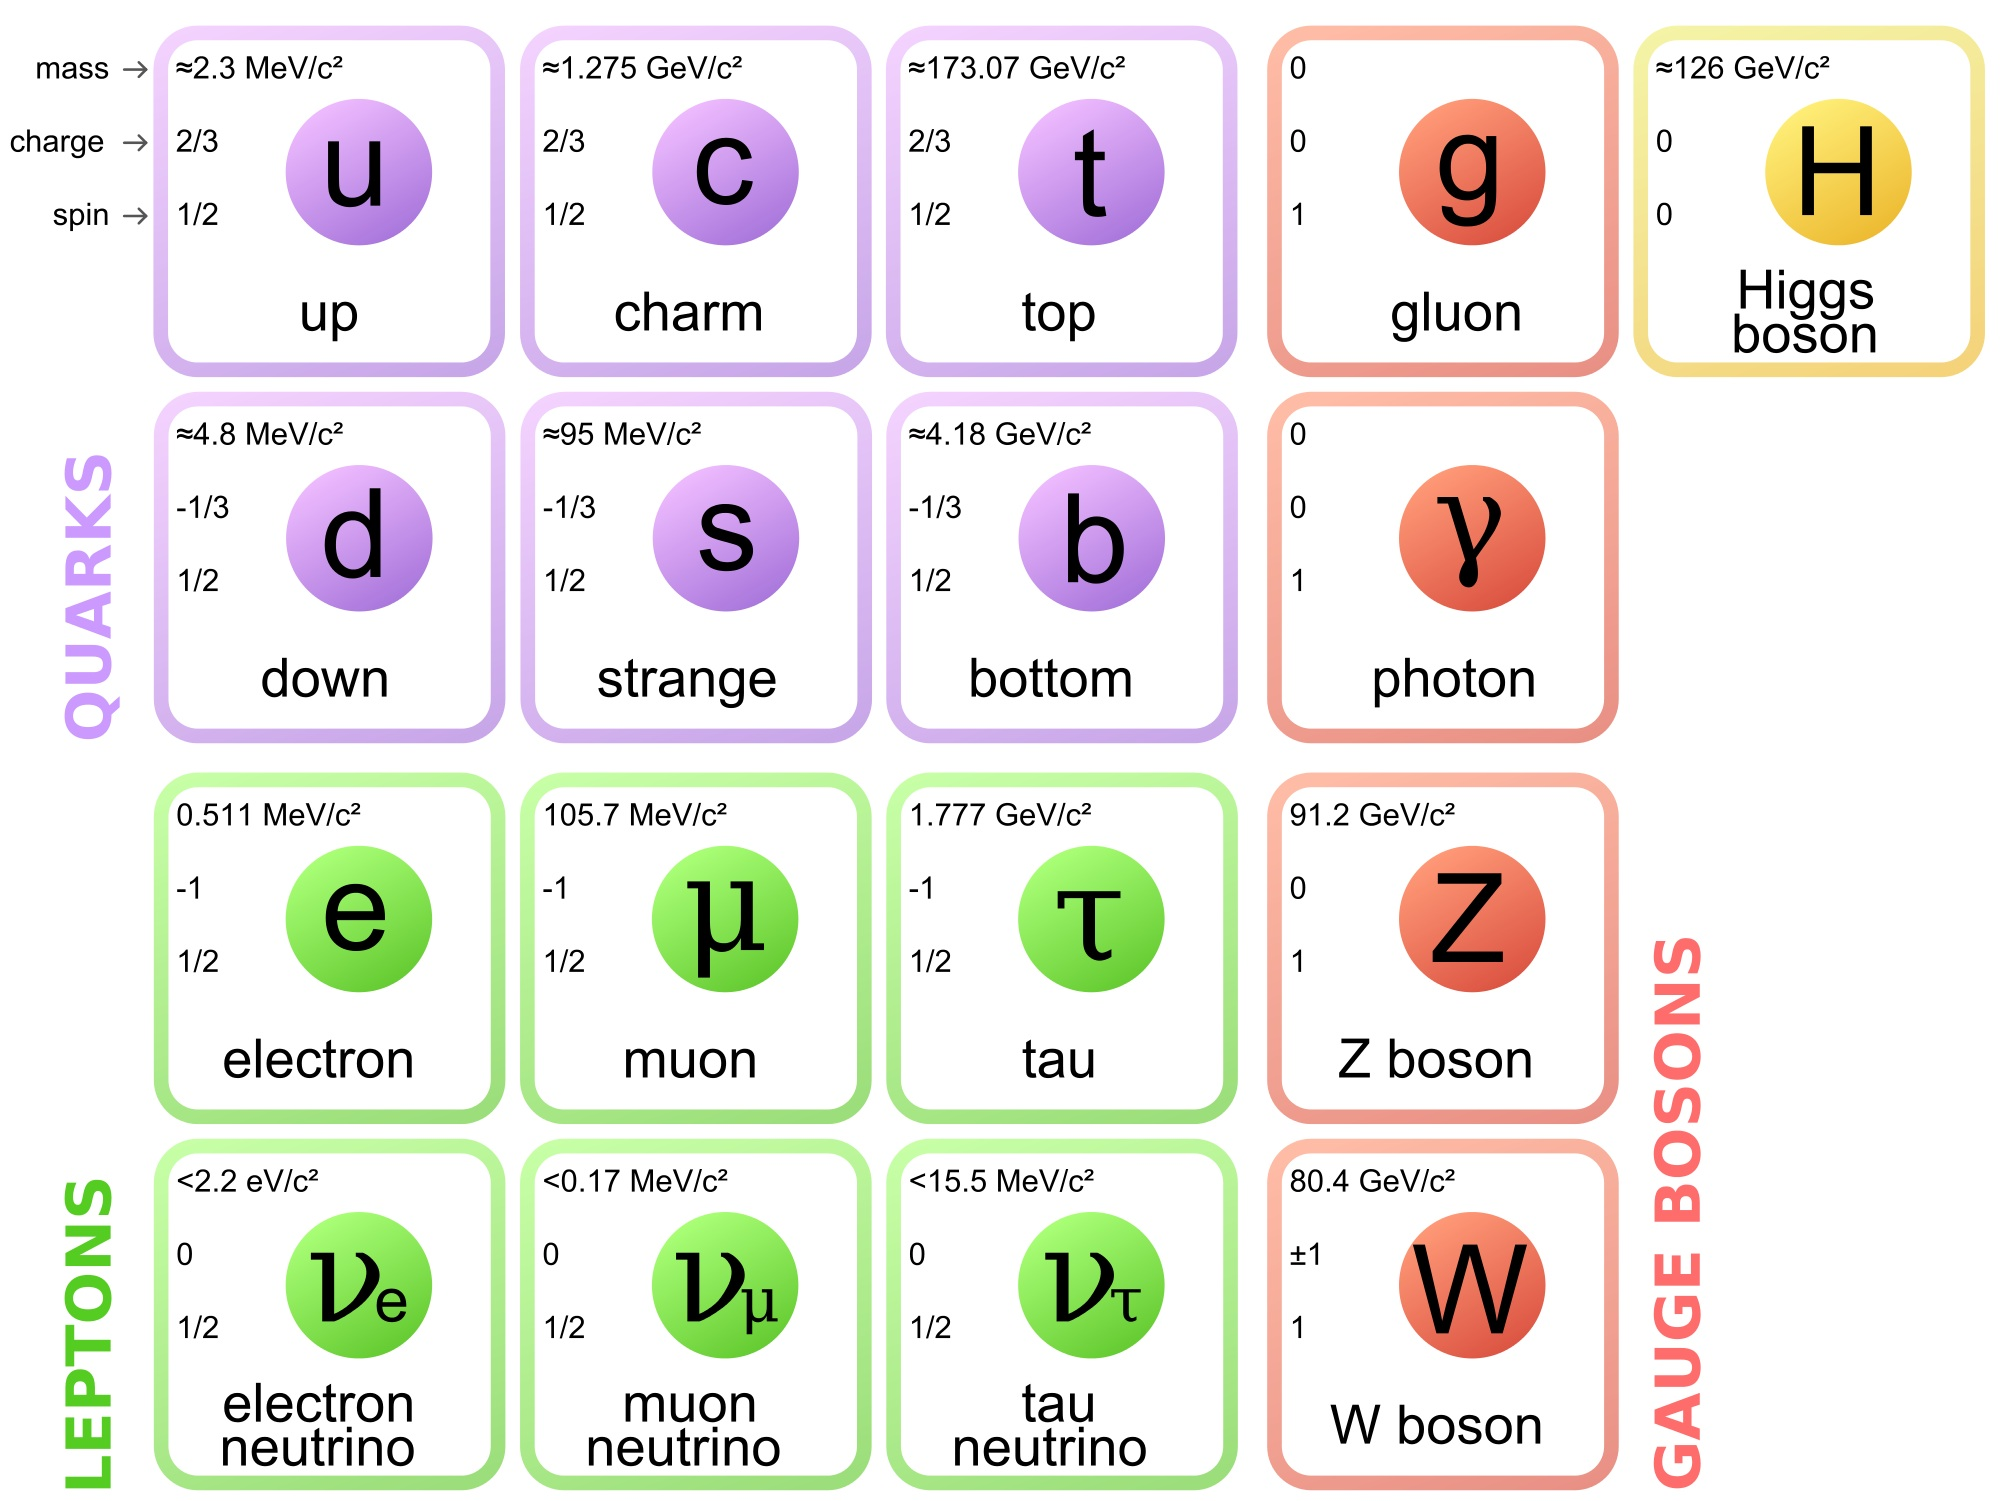
\includegraphics[width=0.70\textwidth]{standard-model.jpg}
	\caption{Standard Model of particle physics.}
	\label{standard-model}
\end{figure}

\section{Antimateria}

Una delle caratteristiche fondamentali delle particelle, lo spin (momento angolare intrinseco), permette di distinguerle in due classi: i bosoni, con spin intero, ed i fermioni, con spin semi-intero. I fermioni rispondono al principio d'esclusione di Pauli, il quale postula che non ci possono essere due fermioni occupanti lo stesso stato quantistico, mentre ciò è possibile per i bosoni: questo dà luce a fenomeni particolari come la superconduttività e la superliquidità.\\
Se si ignora lo spin, l'equazione di Schrödinger può essere facilmente espressa in forma relativistica; partendo dall'energia $ E^2 = m^2 c^4 + p^2 c^2 $ e ricordando le regole di quantizzazione $ E \mapsto i\hbar \frac{\pa}{\pa t}, p \mapsto -i\hbar \nabla $, si ottiene l'\textit{equazione di Klein-Gordon}:
\begin{equation}
	\frac{1}{c^2} \frac{\pa^2}{\pa t^2} \phi(\ve{x},t) - \lap \phi(\ve{x},t) + \frac{m^2 c^2}{\hbar^2} \phi(\ve{x},t) = 0
	\label{eq:7.1}
\end{equation}
dove $ \phi(\ve{x},t) $ è un campo scalare. Per trattare particelle dotate di spin, è necessario trovare altre equazioni. Per particelle con $ s = \frac{1}{2} $, descritte da uno spinore $ \psi $ a quattro componenti, si trova l'\textit{equazione di Dirac}:
\begin{equation}
	i \gamma^{\mu} \pa_{\mu} \psi - \frac{mc}{\hbar} \psi = 0
	\label{eq:7.2}
\end{equation}
dove le matrici $ \gamma $ sono legate alle matrici di Pauli:
\begin{equation*}
	\gamma^0 \equiv
	\begin{bmatrix}
		\tens{I}_2 & 0 \\ 0 & \tens{I}_2
	\end{bmatrix}
	\qquad \qquad
	\gamma^k \equiv
	\begin{bmatrix}
		0 & \sigma_k \\ -\sigma_k & 0
	\end{bmatrix}
\end{equation*}
La prima grande conseguenza dell'equazione di Dirac è che, risolvendola per elettroni liberi, si trovano due soluzioni: una con energia positiva ed una con energia negativa. Dato che nel mondo reale tutte le energie sono positive, essendoci un'energia minima per le particelle costituita dalla loro massa a riposo, Dirac spiegò la soluzione ad energia negativa tramite l'idea del \textit{Fermi sea}: oltre agli stati ad energia positiva, esistono anche stati speculari ad energia negativa che sono normalmente tutti occupati, così che le particelle reali possano avere solo energie positive. Può capitare però che, con eccitazioni sufficientemente energetiche, una particella nel mare di Fermi venga portata in uno stato ad energia positiva: il vuoto lasciato nel mare di Fermi è interpretato come una antiparticella, ovvero come una copia della particella reale ma con carica elettrica opposta. Questo è proprio il principio della pair production: un fotone sufficientemente energetico ($ E_{\gamma} > 2m_e = 1022\kev $) può fornire l'eccitazione sufficiente a produrre una coppia elettrone-positrone.\\
Un'interpretazione diversa dell'antimateria sarà poi data da Feynman: le antiparticelle non sono più viste come buchi nel Fermi sea, ma come particelle che si muovono in maniera opposta lungo la direzione temporale: ciò comporta che le antiparticelle hanno la stessa massa delle particelle, ma carica elettrica opposta.

\subsection{Evidenze sperimentali}

Le prime evidenze sperimentali dell'esistenza dell'antimateria si ebbero con lastre fotografiche che, mostrando tracce di ionizzazione, rilevavano fenomeni di pair production.

\paragraph{Positrone}

Il positrone fu osservato per la prima volta da Skobeltsyn nel 1929 durante lo studio di raggi cosmici in una cloud chamber e nel 1932 da Anderson con lo stesso metodo. La scoperta fu confermata nel 1932 da Blacket ed Occhialini in laboratorio. A posteriori, altri sperimentatori in precedenza si sarebbero potuti accorgere della sua esistenza: ad esempio, i coniugi Curie lo avevano osservato, ma senza dargli attenzione lo avevano classificato come un protone.\\
Il positrone è una particella stabile come l'elettrone, ma la sua vita media è comunque estremamente breve ($ \tau \sim 10^{-10}\,\text{s} $) poiché forma immediatamente un sistema con un elettrone nella materia, detto positronio, il quale decade per annichilazione.\\
Un'importante applicazione del positrone è la \textit{Positron-Electron Tomography} (PET), un esame diagnostico per tumori: dato che il positronio decade in due fotoni con $ E_{\gamma} = 511\kev $ emessi in direzioni opposte, facendo accumulare una concentrazione abbastanza alta di un positron-emitting radionuclide in una massa tumorale, è possibile tracciarne con precisione la posizione nel corpo, dato che essa deve trovarsi lungo la linea che congiunge i due fotoni rilevati. Un metodo utilizzato è l'accumulo di $ \ch{^{18}F} $ (decade $ \beta^+ $) misto a glucosio: le cellule tumorali hanno un consumo di zuccheri dieci volte superiore alle cellule normali.

\paragraph{Antiprotone}

L'antiprotone fu osservato nel 1955 al Bevatron, un sincrotrone per protoni a Berkley, da Chamberlain e Segrè: ciò confermò che ogni particella aveva una corrispondente antiparticella identica ad essa ma di carica elettrica opposta. Il delay di 20 anni tra le due scoperte fu dovuto al fatto che la massa del protone è quasi 2000 volte quella dell'elettrone, dunque anche le energie necessarie alla produzione di antiprotoni lo sono.\\
Anche gli antiprotoni sono stabili ma short-lived, sempre a causa dell'annichilimento da contatto con materia ordinaria.\\
Poco dopo la conferma dell'esistenza dell'antiprotone, nel 1956 sempre al Bevatron fu osservato l'antineutrone.

